
\section{Intro}
\label{intro}

Book starts with explaining the relation between magnetism and
\begin{itemize}
	\item Maxwell's Equations
	\item Classical Electron Theory
	\item Quantum Mechanics
\end{itemize}





\subsection{Magnetic Fields: Observation}
\subsubsection{Current-Carrying Wire}

A current, passing through a wire, causes magnetic field around itself. This field conforms with the right-hand rule.


\begin{wrapfigure}{l}{0.25\textwidth}
    \centering
    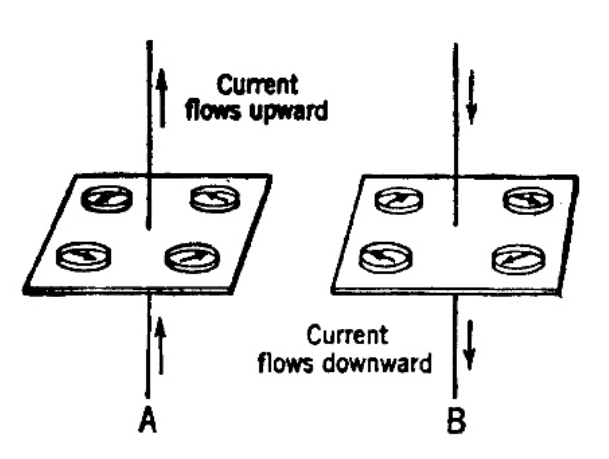
\includegraphics[width=0.25\textwidth]{oersted1.png}
\end{wrapfigure}


\subsubsection{Solenoid}


\begin{wrapfigure}{l}{0.25\textwidth}
    \centering
    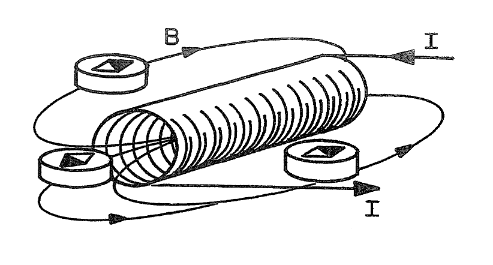
\includegraphics[width=0.25\textwidth]{solenoid1.png}
\end{wrapfigure}

\subparagraph{Earth's magnetic field} is believed to be formed as a result of currents flowing in it's molten core.

\subsubsection{Voltage Induced in a Coil}

According to Lenz' law, change in flux in a coil induces voltage to complement the reduction.
\begin{wrapfigure}{l}{0.25\textwidth}
    \centering
    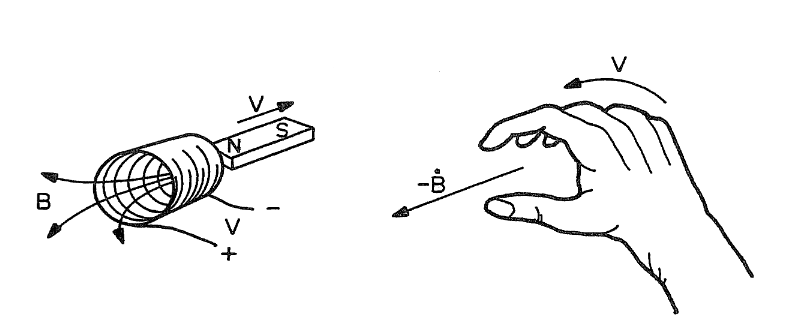
\includegraphics[width=0.25\textwidth]{lenz1.png}
\end{wrapfigure}

\begin{equation}
	v=-\frac{dB}{dt}
\end{equation}


It does not try to complement the diminishing flux such that the flux $\Phi$ passing through the coil is same/constant. According to the law, if the change in flux is small but rapid, this will result with a high induced voltage.

This induced voltage enables the operation of generators and transformers, and a material behavior known as \textit{diamagnetism}.

While Faraday's law tells us the magnitude of the EMF produced, Lenz's law tells us the direction that current will flow.

\begin{equation}
	\mathcal{E}=-\frac{d\Phi}{dt}
\end{equation}



\subsection{Constitutive Relations}

Electric field may cause separation between positive and negative charges within a material. Electric dipole moment is the measure of this seperation, in other terms, polarization measure of this form.

\begin{equation}
	\textbf{p}_{e} = qd \quad [\mathrm{Cm}]
\end{equation}

where $\textbf{p}_{e}$ is the electric dipole moment, $q$ is charge and $d$ is the displacement. This is the equation for one dipole. To achieve a density equation,

\begin{equation}
	\frac{N}{V}p_{e}=np_{e}=P \quad [\mathrm{C/m^{2}}]
\end{equation}

where, $N$ is the number of electric dipoles, $V$ is the volume dipoles take up and $P$ is macroscopic dipole moment density. Vector form of macroscopic dipole moment density \textbf{P} is linked with electric field \textbf{E} as follows, 

\begin{equation}
	P = \chi_{e} E
\end{equation}

where, $\chi_{e}$ is electric susceptibility. Finally, electric displacement field is

\begin{equation}
	\mathbf{D} = \epsilon_{0} \mathbf{E} + \mathbf{P} = \epsilon_{0} \mathbf{E} + \chi_{e} \mathbf{E} =(\epsilon_{0} + \chi_{e}) \mathbf{E} = \epsilon \mathbf{E}
\end{equation}

Now, in a similar manner to electric field $E$, applied magnetic field $H$ provokes responses on materials. A magnetic field causes change in magnetic dipole moment $p_{m} \quad [\mathrm{Am^{2}}]$ of a material. Here, magnetic dipole moment is described as a dipole with infinitesimal size. Magnetization $M$ is defined as macroscopic magnetic dipole moment density, that is 

\begin{equation}
	\frac{N}{V} p_{m} = np_{m} = M \quad [\mathrm{A/m}]
\end{equation}
where, $N$ is the number of magnetic dipoles, $V$ is the volume dipoles take up and $M$ is macroscopic magnetic dipole moment density. Vector form of macroscopic magnetic dipole moment density \textbf{M} is linked with magnetic field \textbf{H} as follows, 

\begin{equation}
	M = \chi_{m} H \quad [\mathrm{A/m}]
\end{equation}

where, $\chi_{m}$ is magnetic susceptibility. Finally, magnetic flux density is is

\begin{equation}
	B = \mu_{0} (H + M) = \mu_{0} (H + \chi_{m} M) =\mu_{0} (1 + \chi{m}) H = \mu H \quad [\mathrm{T}, \mathrm{Wb/m^{2}}]
	\label{eq:magneticFluxDensity1}
\end{equation}

The relation $\mu_{0} \mu_{r} = \mu \quad [\mathrm{H/m}]$ suggests that relative permeability from above relationship is

\begin{equation}
	\mu_{r} = (1 + \chi_{m})
\end{equation}

Magnetic material's response to magnetic field $H$, is magnetization $M$. Here, $H$ is the cause and $M$ is the material effect.
\begin{equation}
	B = \mu_{0} H + \mu_{0} M \quad [\mathrm{T}, \mathrm{Wb/m^{2}}]
	\label{eq:magneticFluxDensity2}
\end{equation}

As can be seen in Eq. \ref{eq:magneticFluxDensity1}, \ref{eq:magneticFluxDensity2}, magnetic flux density $B$ is the overall result including both external flux $\mu_{0} H$ and the materials response $\mu_{0} M$. Faraday's Law states that its the change of magnetic flux density $B$ w.r.t time $-\frac{dB}{dT}$ that gives rise to and electric field $E$ or a voltage $V$. In terms of magnetic circuits, ferromagnetic materials provide a path with low reluctance, much like a low resistance resistor to current. As a result, these materials draw the magnetic flux and amplify it with their magnetization.

\begin{wrapfigure}{l}{0.25\textwidth}
    \centering
    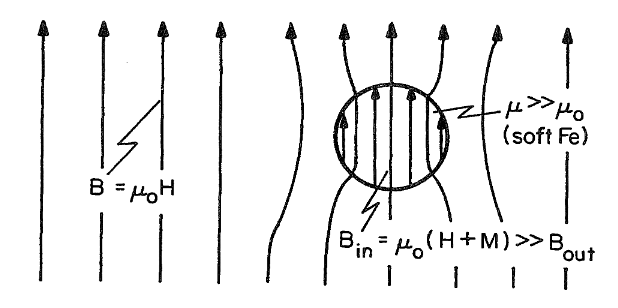
\includegraphics[width=0.25\textwidth]{Bfield_vacuumvsferromag1.png}
\end{wrapfigure}

Note: naval mines (magnetic) utilizes this principle. They are set up as the mine's sensor measures Earth's magnetic field. If a ship (high permeability material $\mu \gg \mu_{0}$) is nearby the mine, magnetic field over the mine is drawn towards the ship. Mine senses this and explodes.



\begin{figure}[h]
    \centering
    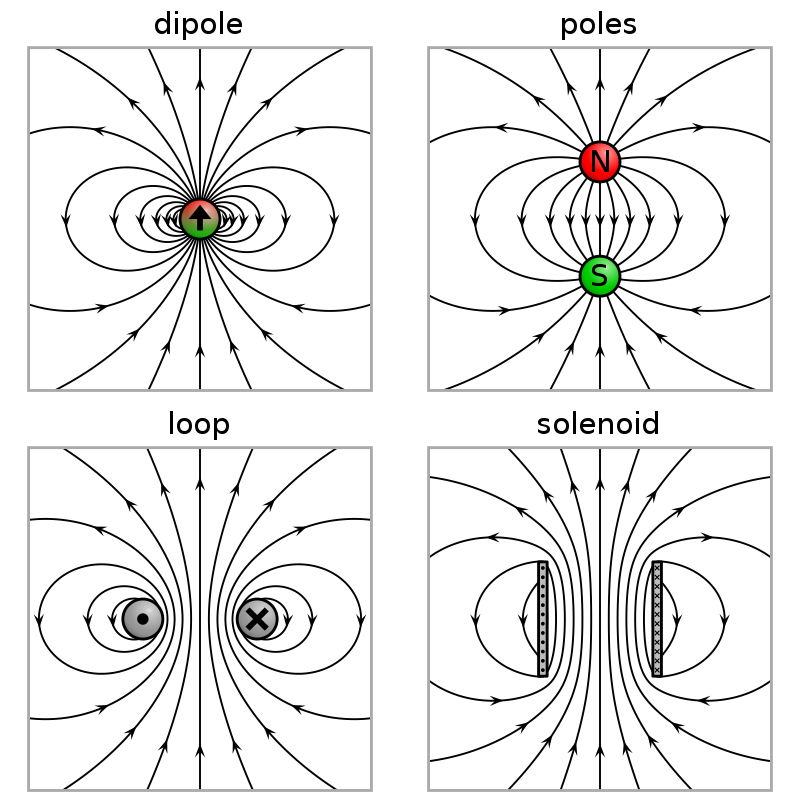
\includegraphics[width=0.75\textwidth]{magneticDipole.png}
\end{figure}


\subsection{Maxwell's Equations}

\subsubsection{Preliminary Mathematics}

Diverging and curling fields are depicted in Fig. \ref{fig:divcurl}. 


Divergence expresses that net flux through an enclosed surface is determined by the sources/sinks enclosed by the surface. In Fig. \ref{fig:divcurl} a, divergence of the field is not zero, meaning that if a surface enclosing the center of the field is considered, there is a field source at the middle, and the net flux is not zero, it is outwards. However, in Fig. \ref{fig:divcurl} b and c, any enclosed surface have a zero net flux, meaning there is no source/sink enclosed by the surface.

In mathematical terms, divergence theorem states that surface integral of a vector field over a closed surface is equal to the volume integral of the divergence over the region inside the surface.

\begin{equation}
	\int \int \int_{V} (\nabla \cdot \mathbf{F})dV = \oint_{S} (\mathbf{F} \cdot \mathbf{n})dS.
\end{equation}

\begin{figure}[h]
    \centering
    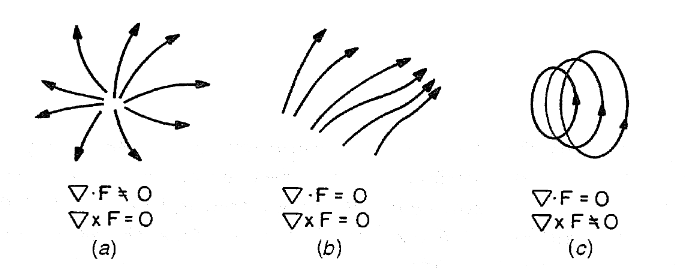
\includegraphics[width=0.75\textwidth]{math_operators1.png}
    \label{fig:divcurl}
\end{figure}


\subparagraph{Gauss's Theorem} $\int (\nabla \cdot \textbf{F})d^{3}x = \int \textbf{F} \cdot d\textbf{A}$


\subparagraph{Stokes Theorem} $\int (\nabla \times \textbf{F}) \cdot \textbf{ dA} = \int \textbf{F} \cdot \textbf{dl}$





\paragraph{Gauss's Law for Electric Fields}

Electric field always moves from a positive charge to a negative charge. In other words, electric charges are sources/sinks for electric fields. There can be electric monopoles, while both positive and negative charges can be obtained individually.

\begin{equation}
	\nabla \cdot \textbf{E} = \frac{\rho}{\varepsilon}
\end{equation}
\begin{eqnarray}
	\int \int \int_{V} (\nabla \cdot \textbf{E}) dV = \frac{1}{\varepsilon} \int \int \int_{V} \rho dV \\
	\oint_{S} \textbf{E} \cdot \textbf{dA} = \frac{1}{\varepsilon} \int \int \int_{V} \rho dV
\end{eqnarray}




\paragraph{Gauss's Law for Magnetic Fields}
\begin{equation}
	\nabla \cdot \textbf{B} = 0
\end{equation}

There is no source for a magnetic flux \cite{Pyrhonen}. All the flux loops are closed. The flux entering an object must also leave the object. These remain to be true unless a magnetic monopole is discovered.
\begin{equation}
	\int \int \int_{V} (\nabla \cdot \textbf{B}) dV = 0
\end{equation}
\begin{equation}
	\oint \textbf{B} \cdot d\textbf{A} = 0
\end{equation}
	 $\nabla \cdot \textbf{B} = 0$ implies there can be no net outflow of $\textbf{B}$ over any  closed surface, therefore no sources of $\textbf{B}$, no magnetic monopoles. Magnetic poles always come in pairs, usually designated north 
and south, called dipoles.



\paragraph{Faraday's Induction Law}
\begin{equation}
	\nabla \times \textbf{E} = -\frac{\partial \textbf{B}}{\partial t}
\end{equation}
\begin{equation}
	\oint_{S} (\nabla \times \textbf{E}) \cdot d\mathbf{S} = -\frac{\partial}{\partial t} \oint_{S} \mathbf{B} \cdot d\mathbf{S}
\end{equation}
\begin{equation}
	\int \textbf{E} \cdot \textbf{dl}= -\frac{d \mathbf{\Phi}}{d t}
\end{equation}

where, $\Phi = B \cdot A$

	Magnetic field $\textbf{B}$ changing in time (time dependent) $-\frac{\partial \textbf{B}}{\partial t}$ causes a spatially rotating electric field $\textbf{E}$.
	Maxwell-Faraday law vs Lenz' law
	A change in current $\textbf{J}$ gives rise to a change in magnetic field $\textbf{B}$. This change in magnetic field $\textbf{B}$ induces an electromotive force $EMF$ opposing the change in current $\textbf{J}$

	
\paragraph{Ampere's Law}
\begin{equation}
	\oint B \cdot dl = \mu_{0} \int J \cdot dA = \mu_{0}J
	\label{eq:AmperesLaw}
\end{equation}
\begin{equation}
	\nabla \times \textbf{B} = \mu_{0}J+\frac{\mu_{0}\varepsilon\partial \textbf{E}}{\partial t}
\end{equation}

Either a current density $\mu_{0}J$ or an electric polarization current $\frac{\mu_{0}\varepsilon\partial \textbf{E}}{\partial t}$ lead to a circulating magnetic field $\nabla \times \textbf{B} \neq 0$.



\subsection{Magnetism and Currents}
\subsubsection{Magnetic Field about a Straight Current-Carrying Wire}

A qualitative measurement for the magnetic flux density $\mathbf{B}$ around a straight current-carrying wire, we use Ampere's law: $\oint B \cdot dl = \mu_{0} \int J \cdot dA = \mu_{0}J$ (neglecting the electric displacement term). Applying this to the problem depicted at Fig. \ref{fig:strcurrentB}, we get

\begin{equation}
	B \cdot dl = 2 \pi R B
\end{equation}

\begin{equation}
	\mu_{0} \int J \cdot dA = \mu_{0}J = \mu_{0} I
\end{equation}

Magnetic flux density $B$ has a uniform magnitude over the line at points equidistant to the wire, therefore, line integral of $B$ gives $2 \pi R B$. Therefore, the resulting magnetic flux density $B$ is ($\mu_{0}$ has a unit of $[\mathrm{H/m}]$)

\begin{equation}
	B = \frac{\mu_{0} I}{2 \pi R} \quad [\mathrm{\frac{HA}{m^{2}}}, \mathrm{\frac{Wb}{m^{2}}}, \mathrm{T}]
\end{equation}

In terms of magnetic field $H = \frac{B}{\mu_{0}}$

\begin{equation}
	H = \frac{I}{2 \pi R}
\end{equation}

Note: through the book by O'Handley [\cite{ohandley_modern_2000}], the term $H$ is used in behalf of magnetic fields sourced by macroscopic currents, e.g. by magnetic charges. The term $B$ is used for magnetic fields when microscopic currents contribute to the flux density, especially in situation where magnetization is important.




\begin{figure}[h]
    \centering
    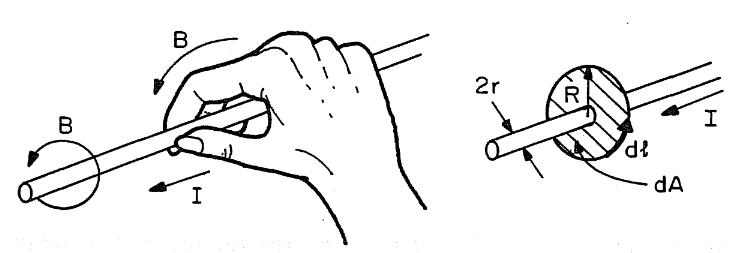
\includegraphics[width=0.75\textwidth]{oersted2.png}
    \label{fig:strcurrentB}
\end{figure}

\begin{eqnarray}
	\textbf{B} = \frac{\mu_{0} I}{2 \pi R} \\
	\textbf{H} = \frac{I}{2 \pi R} \\
	\textbf{H} = \frac{\textbf{B}}{\mu_{0}}
\end{eqnarray}

\begin{eqnarray}
	\nabla \times \textbf{B} = \mu_{0} \textbf{J} \\
	\nabla \times \textbf{B} = \frac{1}{r} \frac{\partial}{\partial r} [r B_{\theta}(r)] = \mu_{0} \textbf{J} \\
	\int_{0}^{R} \{ \frac{\partial}{\partial r}[r B_{\theta}(r)] = \mu_{0} \textbf{J} \} dr \\
	R B_{\theta}(R) = \mu_{0} \textbf{J} \frac{R^{2}}{2} \\
	B_{\theta}(R) = \mu_{0} \textbf{J} \frac{R}{2}
\end{eqnarray}

\begin{eqnarray}
	\textbf{J} = \frac{I}{\pi R^{2}} \\
	B_{\theta}(R) = \mu_{0} \frac{\textbf{I}}{2 \pi R} \\
	\textbf{H} = \frac{B_{\theta}(R)}{\mu_{0}} = \frac{\textbf{I}}{2 \pi R}
\end{eqnarray}



\subsubsection{Moment of a Current Loop}

The source that leads to atomic magnetic moment $p_{m}$ are microscopic current loops inside the material.

To find the magnetic flux density $B$, Ampere's law is utilized to a solenoid, as depicted in Fig. \ref{fig:coilfield1}.
\begin{figure}[h]
    \centering
    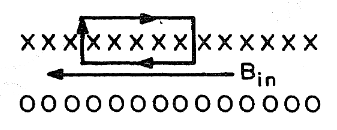
\includegraphics[width=0.25\textwidth]{coilfield1.png}
    \label{fig:coilfield1}
\end{figure}

\begin{equation}
	\oint B \cdot dl = \mu_{0} \int J \cdot dA = \mu_{0} NI
\end{equation}

Here, the book assumes that the $B$ is only non-zero on the integral line inside the solenoid. Therefore, 
\begin{equation}
	\oint B \cdot dl = B_{in}l
\end{equation}
where, $l$ is the length of the solenoid. As a result,

\begin{eqnarray}
	B_{in}l = \mu_{0} NI \\
	B_{in} = \frac{\mu_{0} NI}{l}
	H_{in} = \frac{NI}{l}
\end{eqnarray}

where, the term $\frac{N}{l}$ represents the number of coils the the line of integration encloses, and $I$ is the current each of these coils carry.


\subsubsection{Origin of Atomic Magnetic Moment}

The study done above for a magnetic flux density generated by a solenoid can be seen as the origin of the atomic magnetic moment in a ferromagnetic material. If external magnetic field is zero, i.e. $H=0$, then the magnetic flux density $B$ is
\begin{eqnarray}
	B = \mu_{0} (H+M) = \mu_{0}M \\
	M = (\frac{N}{l})I
\end{eqnarray}

where, magnetization $M$ is replaced by magnetic field $H$ stated as the field resulting from a solenoid. Furthermore, $M=np_{m}$ and $n=\frac{N}{V}=\frac{N}{Al}$. Therefore,

\begin{eqnarray}
	M = \frac{N}{Al} p_{m} = \frac{N}{l}I \\
	p_{m} = AI
\end{eqnarray}


\paragraph{Calculating Magnetism in Hydrogen Atom w.r.t. Bohr Model} sourced by electron intrinsic angular momentum (spin of electrons)

According to the discussion above, magnetic moment of a hydrogen atom with 1 electron is $p_{m} = AI$, where $A$ is the area the electron circulates and $I$ is the current representation of the electron. The area can be found by $\pi r_{0}^{2}$ and and the current can be stated as $I = e(\frac{\omega}{2 \pi})$. These are according to Bohr's atomic model and the resulting values are mere approximations.

Angular velocity of the electron can be stated as $\omega = \frac{v}{r_{0}}$, and the current becomes $I = e \frac{v}{2 \pi r_{0}}$. Electron's velocity can be derived from its energy, that is $E = \frac{1}{2}mv^{2}$. Resulting magnetic moment is

\begin{eqnarray}
	\mu_{m} = p_{m} = IA && \approx e(\frac{\omega}{2 \pi} \pi r_{0}^{2}) \\
	&& \approx e(\frac{v}{2 \pi r_{0}} \pi r_{0}^{2}) \\
	&& \approx 5.7 \times 10^{-24} \quad [\mathrm{Am^{2}}]
\end{eqnarray}

where, $E$ is the electronic energy of the 1s electron in hydrogen. If a hydrogenic material with $n \approx 10^{29}/m^{3}$ atoms per unit volume is considered, with each atom behaving like a magnetic dipole. Then the magnetization can be calculated as

\begin{eqnarray}
	M = n\mu_{m} = 5.7 \times 10^{5} \\
	B = \mu_{0} (H + M) = \mu_{0} M = 0.72 \quad [\mathrm{T}]
\end{eqnarray}

This is the case in which all the atoms are aligned towards the same direction. This value is called the saturation magnetization $B_{s} = \mu_{0} M_{s}$. The books states that the saturation magnetization $B_{s}$ is about $2.2[\mathrm{T}]$ for Fe, $1.7[\mathrm{T}]$ for Co and $0.6[\mathrm{T}]$ for Ni.


\subsection{Types of Magnetism}

\subsubsection{Weak Magnetism}

Let's take the following equality into consideration:

\begin{equation}
	B = \mu_{0} (H+M) = \mu_{0}H + \mu_{0}M
\end{equation}

Here, the resulting magnetic field has two components. $\mu_{0}H$ component is due to the magnetic field intensity applied externally, and $\mu_{0}M$ component is due to the alignment of atomic magnetic moments within the material.

Magnetic susceptibility $\chi_{m}$ is usually the indicator for weak magnetic responses. Weak magnetic responses occur in materials with susceptibility between $\pm 10^{-4}$ to $10^{-6}$. In these type of materials, majority of the magnetic field $\textbf{B}$ is sourced by the applied magnetic field intensity $\textbf{H}$ and the remaining part is sourced by the magnetization 	$\textbf{M}$. This is because the magnetic moments are not fully, not even significantly aligned. (For hydrogen, magnetization sources the magnetic field of $1$ T when fully aligned, $10^{-6}$ T when not aligned). This is because of the thermal energy in the material, $k_{B}T$.

The potential energy $U$ of the magnetic moment $\mu_{m}$ in an applied magnetic field $B$ is

\begin{equation}
	U = -\mu_{m} \cdot B
\end{equation}

Additionally, thermal energy at room temperature is $k_{B}T$. If, the magnetic energy is small relative to thermal energy, then the field presents a weak, linear effect on aligning the moments.


\subsubsection{Ferromagnetism}

Ferromagnetic materials are characterized by a long-range ordering of their atomic moments, even in the absence of an external field \cite{O'Handley}. This ordering, spontaneous alignment of magnetic moments, is observed to vanish above a certain temperature, called Curie temperature $T_{C}$.


\begin{figure}[h]
    \centering
    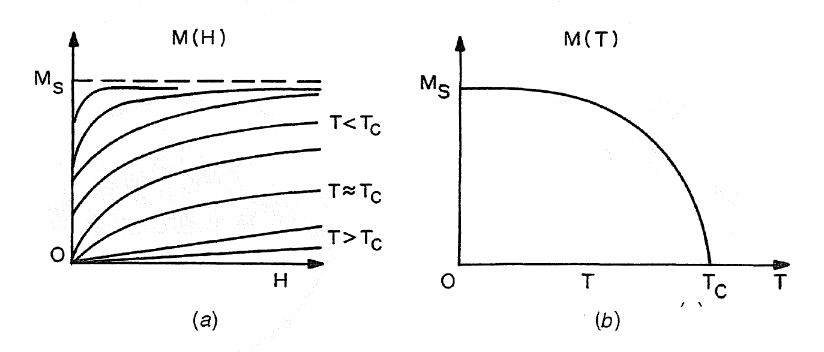
\includegraphics[width=0.75\textwidth]{curie_temperature1.png}
\end{figure}


Relative magnetic permeability $\mu_r=\frac{\mu}{\mu_{0}}=1+\chi_{m}$ is used to describe magnetic response of ferromagnetic materials to magnetic field intensity $H$. 

In ferromagnetic materials, relatively small values of magnetic field intensity $H$ (e.g. $H \approx 100$ A/m) lead to high magnetic field $B$ (e.g. $B=1-2$ T) values.


\subsubsection{Antimagnetism and Ferrimagnetism}


\subsection{Technical Magnetic Materials}

\subsubsection{B-H Loops and Magnetic Domains}

\begin{figure}[h]
    \centering
    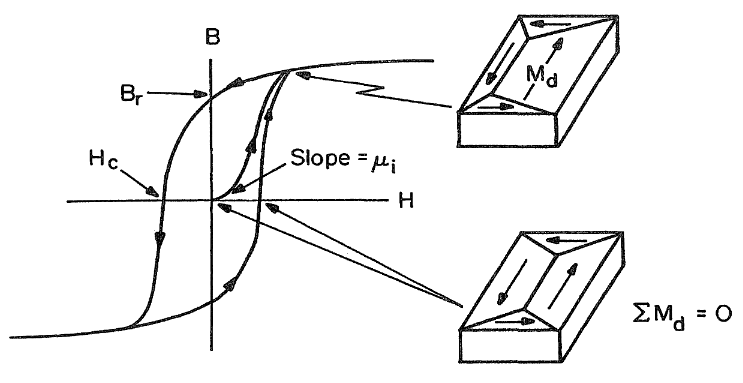
\includegraphics[width=0.75\textwidth]{BH_loops_magneticdomains1.png}
\end{figure}

Starting with a magnetic material at demagnetized state, that is $B=0,H=0$. Increasing the applied magnetic field, applying a weak field to the material leads to certain motions on domain walls such that volume of the domains having the largest component of magnetization $M$ parallel to applied field $H$. Initial permeability $\mu_{i}=(B/H)_{H \approx 0}$ is defined from the initial induction $B$ produced in response to the weak magnetic field intensity $H$. Initial permeability $\mu_{i}$ can be as high as $10^{-1}$ ($\mu_{0} \mu_{r} = \mu_{i}, \mu_{r} \approx 10^{5}$) in some materials. At magnetic field intensities $H$ a little higher, materials permeability increases to its maximum $\mu_{max}$. At this point, the domain wall motion is at its peak. At higher magnetic field intensities $H$, when this motion is finished, there often remain domains with nonzero magnetization orthogonal to the applied field. Magnetization in these domains must also be rotated towards the applied field to achieve minimum potential energy. When these two motions: domain wall motion and orthogonal magnetization rotation are finished, the material comes to a static state of magnetic saturation, where $B_{s} = \mu_{0} (H+M_{s})$.

Now, as the applied magnetic field intensity $H$ decreases, magnetization rotates back to its easy direction first. Rotation is generally a lossless process, without hysteresis. As $H$ decreases further, domain walls recede. Here, the domain walls jump abruptly from one local minimum energy to the next. This is called Barkhausen jumps. During domain wall motion, energy is lost. Therefore, domain wall motions (Barkhausen jumps) are lossy, irreversible processes. As a result, B-H loop opens up (area between the curves for increasing and decreasing magnetic field intensity increases), that is called hysteresis, when lossy magnetization processes are involved. When the applied magnetic field intensity decreases to zero, induction remaining in the material is called residual induction $B_{r}$, and magnetization remaining in the material is called remanence magnetization $M_{r}$. An magnetic field intensity shall be applied to the material in reverse direction, to get such magnetized material to present a magnetic field $B=0$ again. This reverse field is called coercive field $H_c$. It can be seen as a measure of how easy to get the material magnetized. The field needed to restore magnetization $M$ to zero is called intrinsic coercivity $H_{c,intrinsic}$.


\begin{figure}[h]
    \centering
    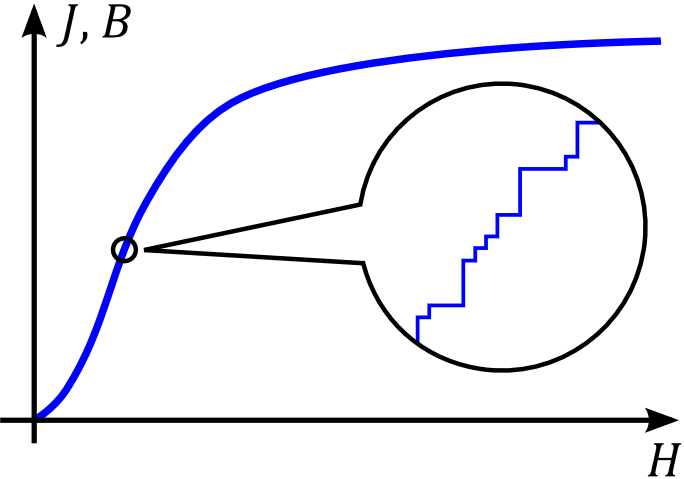
\includegraphics[width=0.35\textwidth]{barkhausen1.png}
\end{figure}


\subsubsection{Soft Magnetic Materials}

Soft magnetic materials are classified as materials in which the domain wall motion and domain magnetization rotation occurs in weak fields (relatively low magnetic field intensities), e.g. $H_{c} \leq 10^{3}$ A/m.

Note: Earth produces a magnetic field of $0.4$ Oe, or $30$ A/m.


\subsubsection{Hard Magnetic Materials}


Some magnetic materials, once magnetized, resist demagnetization. These materials may have defects which strongly impede domain wall motion, or they may consist of single domain particles with high magnetic anisotropy that the direction of magnetization changes with very large fields. These materials are called hard magnets, or permanent magnets. Because they  resist demagnetization in the  presence 
of a  negative field, hard magnets exert a  repelling  force  against  the  source 
of a  negative  imposed field. Thus, permanent  magnets store energy  like a spring;  they excert a  restoring force without contact. The energy stored in a permanent magnet is related to the area inside the  second quadrant of the B-H loop. The (BN),,, quality factor commonly used to rate permanent magnets is the maximum value 
of the BM product  along the B-H   curve in  second quadrant. Hard magnets are used  in many motors and actuators; they also find applications in  frictionless bearings,  microwave  generators, and lenses for charged particle machines.

\subsubsection{Demagnetizing Field}
\label{sec:demagnetizingField}

The answer is in the examination of airgap surfaces. Free poles occur at the surfaces of magnetized materials from which the flux passes through. These free poles (north) emanate magnetic field $H$ which tries to reach to free poles (south). Here, magnetic pole strength per surface area is given as

\begin{equation}
	\sigma = \textbf{M} \cdot \textbf{n}
\end{equation}

where, $\textbf{M}$ is magnetization and given as $= np_{m} = \frac{N}{V} P_{m}$, and $\textbf{n}$ is the normal vector.

Magnetic pole strength per surface area $\sigma$ sets up magnetic field on both sides of a surface. Answer to the question that is asked before, why magnetic fields at the airgap and on the PM are in opposite direction, is here. From the surface with north poles emerges magnetic field $H$ to go to the opposing airgap surface, which is with south poles. Some magnetic field goes through the airgap, resulting with airgap flux, and some go through the PM material. Magnetic field emanates through the material is called demagnetizing field.

\begin{figure}[h]
    \centering
    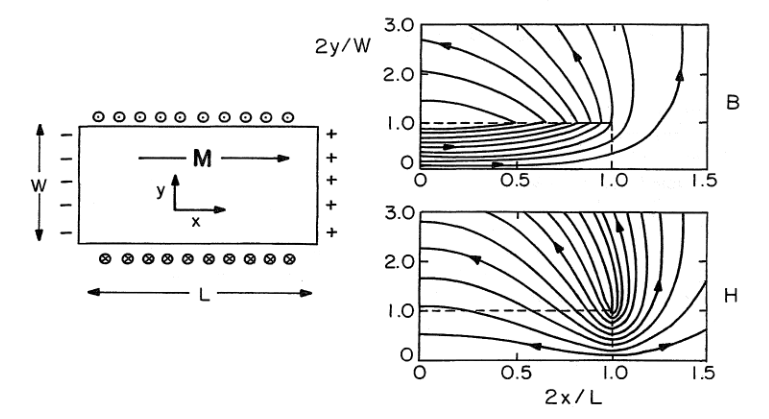
\includegraphics[width=0.85\textwidth]{demagnetizingField1.png}
    \label{fig:demagnetizingField1}
\end{figure}

As can be seen in Fig. \ref{fig:demagnetizingField1}, the magnetic flux density $B$ obeys the Ampere's law, is formed according to current loops depicted on top and bottom of the material.

